\section{Discussion}
    \begin{figure}[ht]
        \centering
        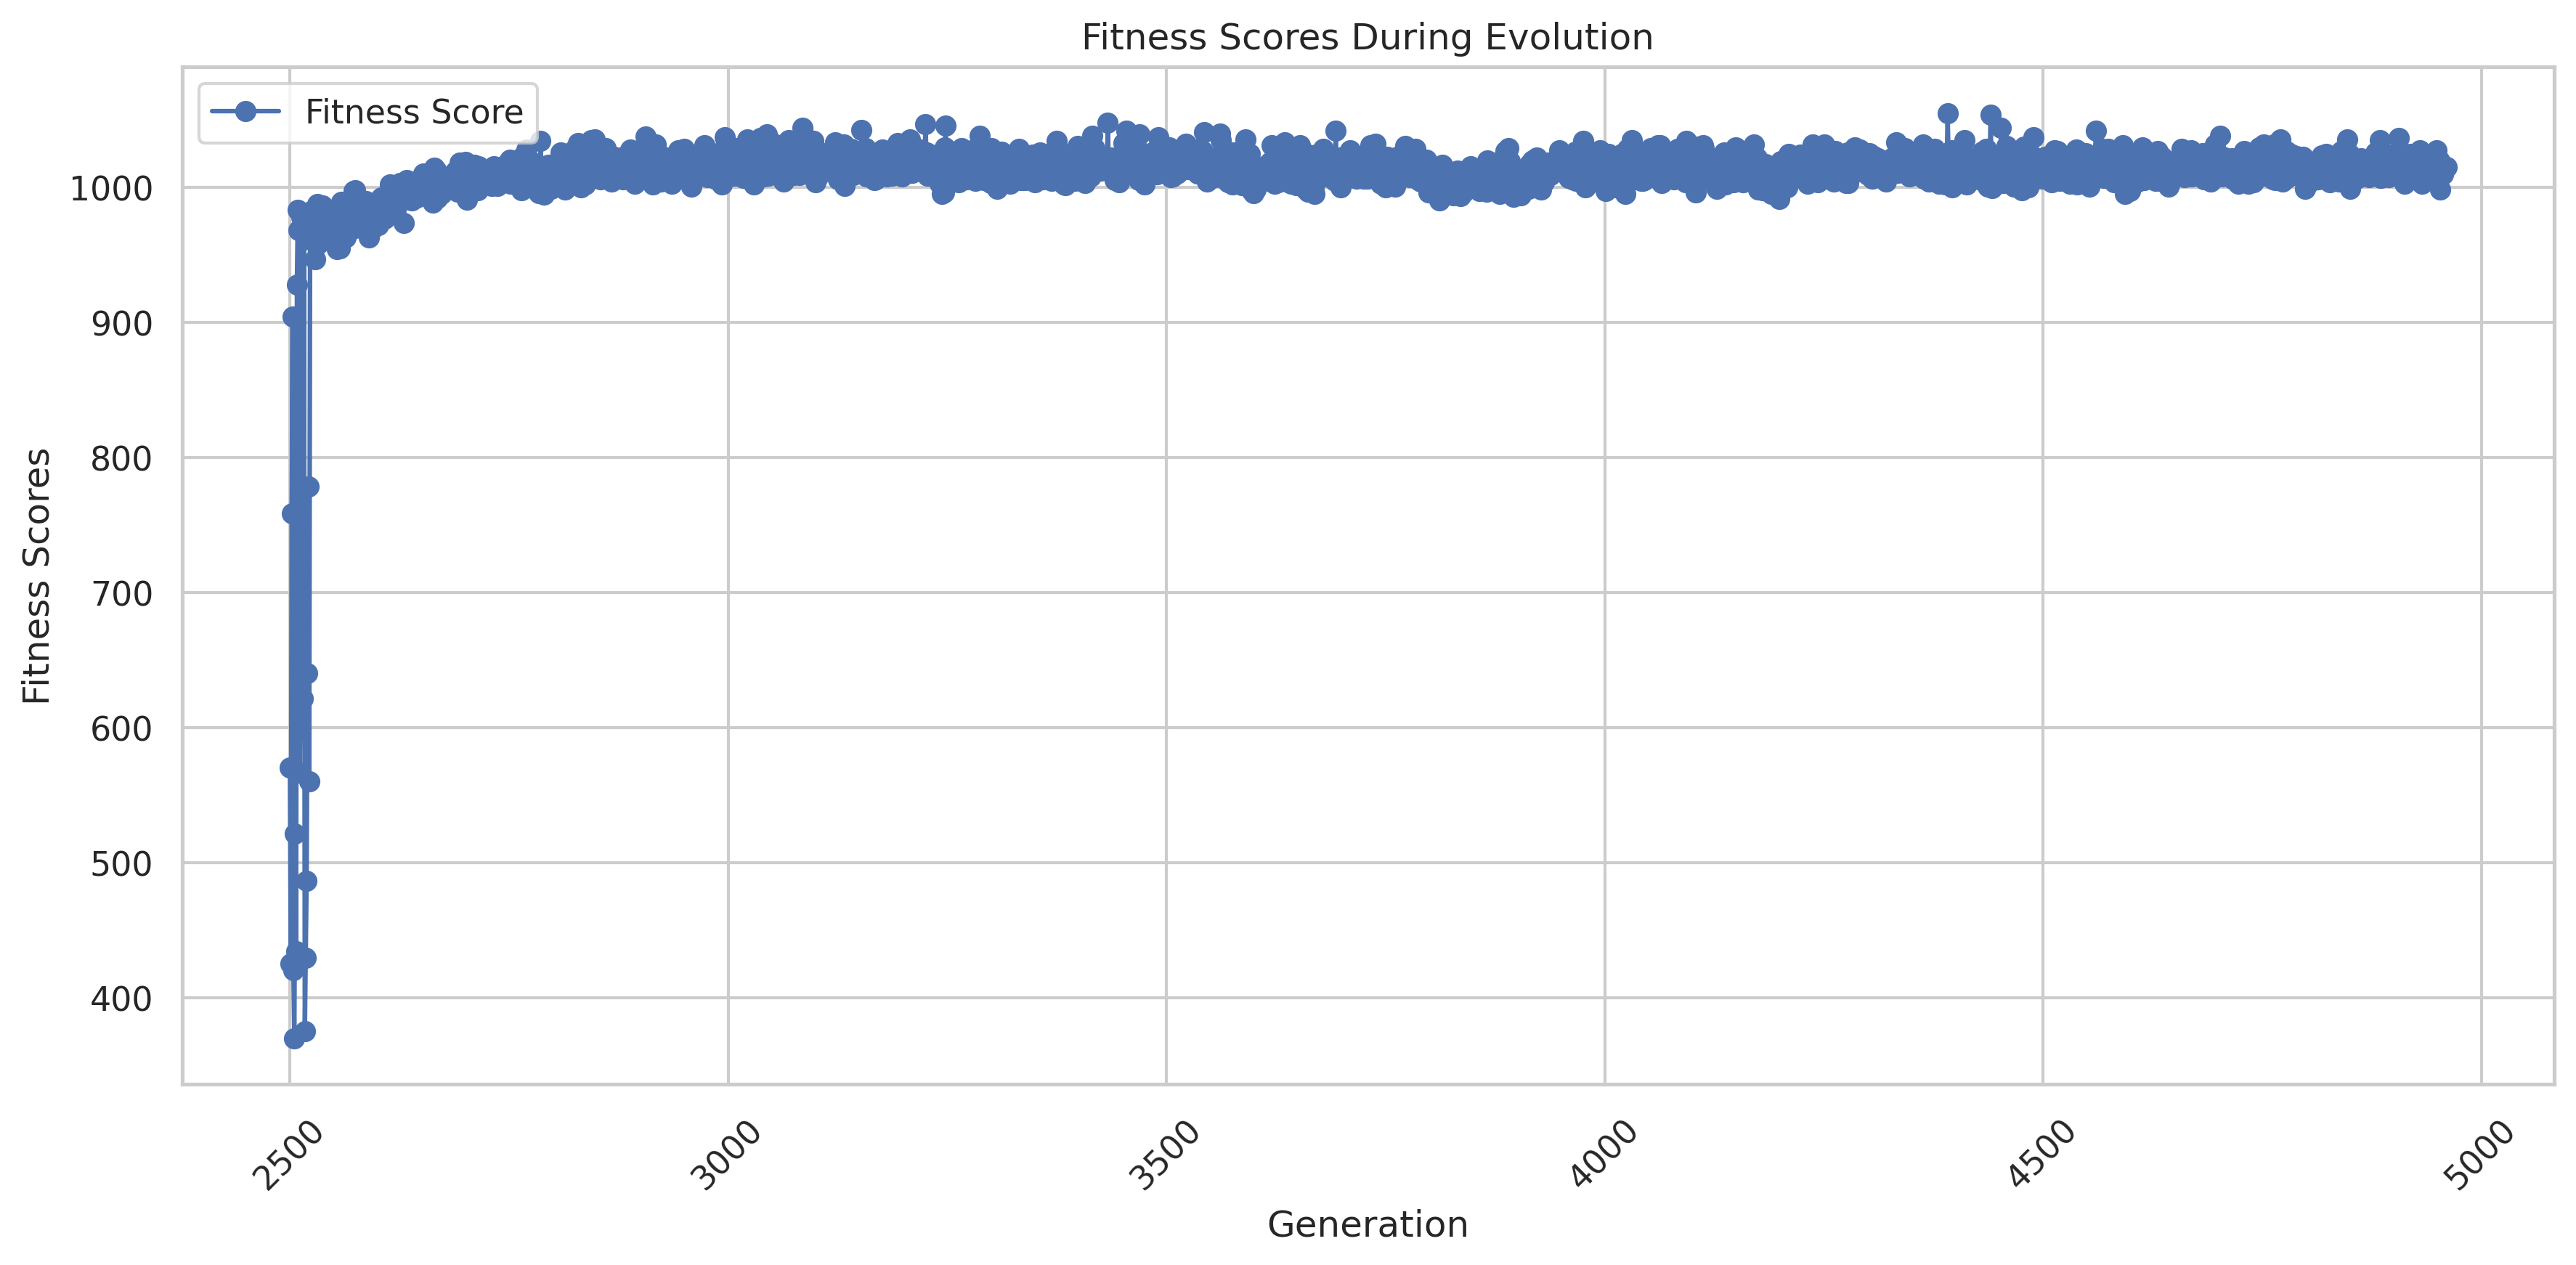
\includegraphics[width=\linewidth]{resources/specialist_1_2835/fitness_score_metrics_plot.png}
        \caption{Experiment 3 - This plot shows the fitness scores of an evolved MC-pair on the rough terrain environment with block size 1 and floor height 0.9 over 5000 generations.}
        \label{fig:eval_plot_spec_1}
    \end{figure}

The results of the three experiments reveal several insights into the evolution of generalist MC-pairs. Both interpolation and extrapolation tests reveal that the method employed in this study improves generalizability, enabling the MC-pair to perform on both in-distribution testing and out-of-distribution testing.

Interestingly, the specialists underperformed compared to the generalist MC-pair, contrary to what was expected. It is generally hypothesized that specialists outperform generalists. Consider the evolution of the MC-pair, visible in Figure~\ref{fig:eval_plot_spec_1}, evolved over 5000 generations in the rough terrain environment with a block size of 1 and a floor height of 0.9, obtaining scores around the 1000. In contrast, the generalist controller in experiment 2, scored around 2000 in the same environment. This indicates that training the MC-pair in a static environment, especially if the environment is more challenging, is counterproductive. Multiple factors may explain this underperformance. One option is that the environment is simply too challenging, and variability helps the search for effective MC-pairs, similar to what curriculum learning does. Another potential reason is that the search converges prematurely to a suboptimal solution. In this paper \cite{Emma_Stensby_2021}, curriculum learning was applied to tackle the problem of premature convergence when evolving MC-pairs, successfully addressing this problem. This also explains the underperformance of partition 2 in Figure~\ref{fig:experiment2}, where partition 2, only had two environments to train on, being less variable.

In our experimental design, the starting position of the ant was set to one unit above the maximum floor height of the environment. This adjustment ensured that the ant would not spawn in the ground. However, this configuration introduced a minor delay in the ant's initial contact with the ground in environments with lower floor heights, thereby slightly disadvantaging it. However, this was not significantly noticeable in the results, as the environments with lower floor heights are inherently easier than those with higher floor heights.

Another notable aspect of our experiment was the symmetry in the ant's morphology, which rendered modifications to  specific legs arbitrary. For instance, altering the length of legs 1 and 2 while shortening legs 3 and 4 results in the exact morphology to its reverse. This symmetry significantly reduced the number of novel morphologies the ant could evolve into drastically, despite having a relatively large search space. To enhance the potential for more novel morphologies in future experiments, we could create and evolve the legs during the evolutionary process and include variations in the attachment points of the legs on the ant's torso. 

Given the diverse range of environments, each with unique challenges and complexities, employing TWEANNS might offer advantages over static ANN architectures. By using TWEANNS, it would be possible to evolve ANN structures specifically designed to generalize on all environments.

The methodology employed in this paper does not have an explicit objective function for generalizability; however, it emerges as a side effect of the applied methods. A future approach could involve making generalizability the primary objective. This approach would require increased computational resources, because of the need to assign a generalist score across the entire population, as also highlighted by Triebold et al. \cite{Corinna_Triebold}.

Regarding the environment generation, each type of environment was generated with just two dimensions. Adding additional dimensions will increase the variability of these environments, potentially further improving generalizability. Beyond solely structural modifications to the environment, incorporating variables such as changes in gravity or variations in the drag force of the ground could provide more insights into the evolution of MC-pairs, better mimicking real-world scenarios. Additionally, investigating the step size variable, exploring its trade-offs and potentially identifying an optimal step size value, which could result in decreasing the size of the training sets, thereby decreasing the generalist score evaluation.